%        File: chameleon-arch-2.tex
%     Created: Mon Jan 04 08:00 PM 2016 C
% Last Change: Mon Jan 04 08:00 PM 2016 C
%
\documentclass{standalone}

\usepackage{tikz}
\usetikzlibrary{arrows.meta, positioning, shapes, calc, backgrounds, fit}

\begin{document}
\begin{tikzpicture}[connection/.style = {>=Stealth, <->, brown, dashed, line width = 3pt}]
  % background: china map
  \node (china-map) [opacity = 0.20] {
\includegraphics[scale = 0.40]{figs/china-outline-blue.png}};

  % partition-left, partition-right, partition-below
  \node (partition-left) [] at (-6.5, 1) {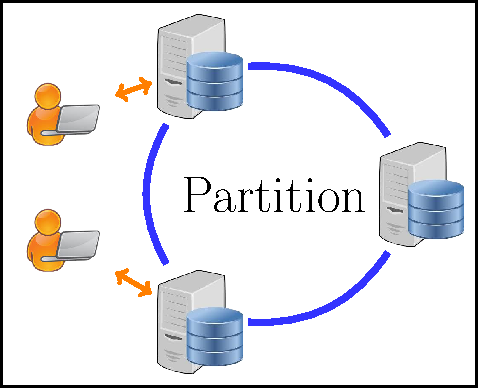
\includegraphics[scale = 0.80]{figs/partition.pdf}}; 
  \node (partition-right) [] at (6, 3.5) {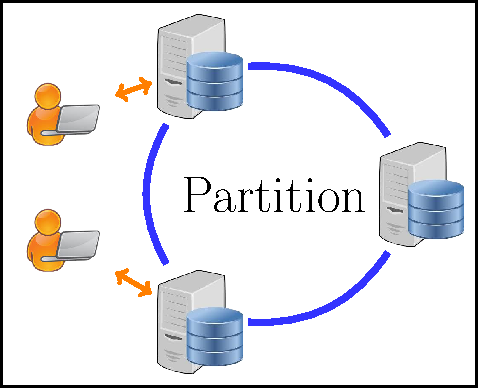
\includegraphics[scale = 0.80]{figs/partition.pdf}}; 
  \node (partition-below) [] at (1.5, -5) {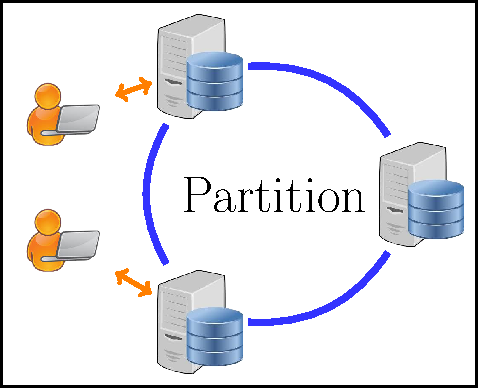
\includegraphics[scale = 0.80]{figs/partition.pdf}}; 

  % connections among partitions
  \draw [connection] (partition-left) to (partition-right); 
  \draw [connection] (partition-right) to (partition-below);
  \draw [connection] (partition-below) to (partition-left);

  % replication 
  \node (replication) [font = \Huge, align = center] at (0.5, 0.0) {\textbf{Wide-area}\\[3pt]\textbf{Replication}};

  % master-slave for one partition
  \begin{scope}[circled/.style = {draw, circle, loosely dashed, cyan, ultra thick, outer sep = 5pt, minimum size = 2.0cm}, 
    conn/.style = {dash pattern = on 15pt off 8pt, cyan, line width = 1.5pt}]
  \node (ms-left) [circled] at (-4., 1) {};
  \node (ms-right) [circled] at (5.5, 1.7) {};
  \node (ms-below) [circled] at (4., -5.0) {};

  \node (master-slave) [below right = 1.5cm and -1.5cm of partition-right] {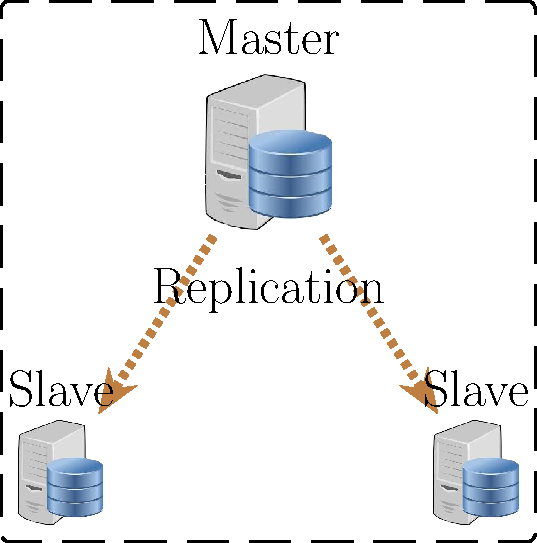
\includegraphics[scale = 0.80]{master-slave.pdf}};
  \draw [conn] (ms-left) to (master-slave);
  \draw [conn] (ms-right) to (master-slave);
  \draw [conn] (ms-below) to (master-slave);
  \end{scope}
\end{tikzpicture}
\end{document}
